\chapter{Diversiteit in game content}
\label{ch:diversiteitingamecontent}
De corporate learning afdeling van \&ranj houdt zich vooral bezig met het maken van narrative games op maat. Het bedrijf heeft een ontwikkelomgeving opgezet waarin narrative games efficiënter ontwikkelt kunnen worden. In dit hoofdstuk wordt er nader in gegaan op de story- en dialog editor. Dit zijn applicaties waarin het narratief achter het spel zonder enige programmeerkennis geschreven kan worden. 

De huidige editors moeten telkens aangepast worden om nieuwe game content te ondersteunen die geïntroduceerd wordt door de projecten op maat. Dit hoofdstuk stelt een oplossing voor waarmee de editors op een flexibele manier om kunnen gaan met de diversiteit aan game content.

\section{Story- en dialog editor}
Tijdens het ontwikkelproces van een narrative game werken game designers, visual designers en programmeurs nauw samen. Om game designers het verhaal te laten schrijven en hierin visuals te verwerken zijn er twee editors opgezet; de story- en dialog editor. De programmeurs kunnen vervolgens de game engine aanpassen om het geschreven verhaal te interpreteren, om zo het verhaal te visualiseren in het spel.

\begin{wrapfigure}{r}{0.35\textwidth}
    
\includegraphics[width=0.33\textwidth]{Graph}
    \caption{Visuele representatie van een graaf.}
    \label{fig:graph}
    \centering
\end{wrapfigure}

Game designers maken gebruik van de visual scripting interface die de editors bieden. Deze visual scripting interface bestaat uit visuele componenten die dienen als bouwblokken waaruit het verhaal is opgebouwd. Door deze bouwblokken op het canvas te plaatsen en met elkaar te verbinden kan er een verhaal worden geschreven. Zo zijn er bouwblokken waarmee conditionaliteit toegepast kan worden en bouwblokken die een content type vrij laten komen. Content typen zijn kleine datastructuurtjes met een betekenis in het verhaal. Een voorbeeld van zo’n content type is ‘text content’. Deze bevat een tekst die getoond zal worden in het spel. In \autoref{sec:contenttypen} zal er dieper worden ingegaan op content typen.

In de editors wordt een verhaal gerepresenteerd als een graph, in het Nederlands graaf genoemd\cite{Aho1983}. Een graaf bestaat uit nodes en edges, zoals weergeven in \autoref{fig:graph}. De nodes zijn de bouwblokken en de edges de verbindingen tussen deze bouwblokken. Aan de editors is het goed terug te zien dat het verhaal gerepresenteerd wordt als een graaf (\autoref{fig:storyeditorsimplegraph}).

In \autoref{ch:formalism} wordt er dieper ingegaan op het interpreteren van deze verhaal graaf. 

\begin{figure}[H]
    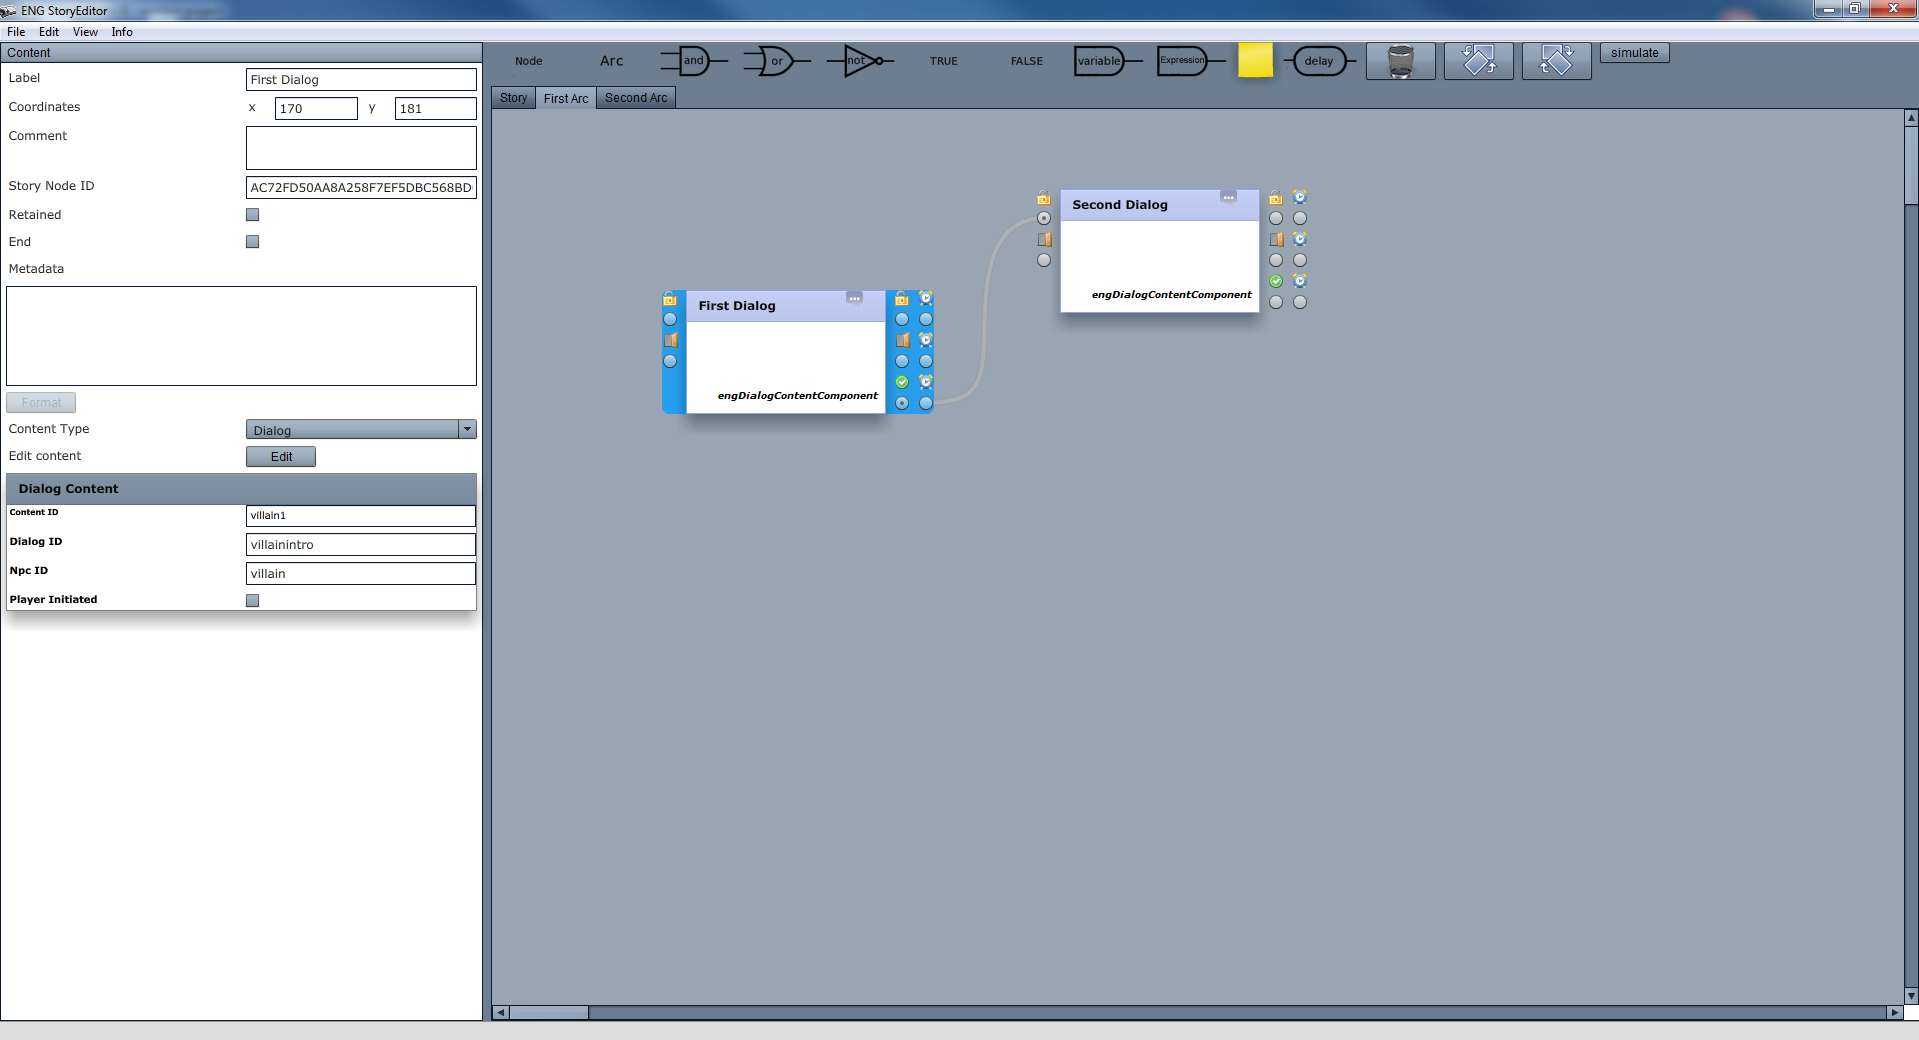
\includegraphics[width=\textwidth]{StoryEditor_SimpleStory_2dialogs}
    \caption{Een simpel verhaal gemaakt in de story editor}
    \label{fig:storyeditorsimplegraph}
    \centering
\end{figure}

\pagebreak

\section{Content typen}
\label{sec:contenttypen}
Iedere game bestaat uit game content. Dit is een verzamelnaam voor alle teksten, media en mechanieken die zich binnen het spel bevinden. Om onderscheid te maken tussen game content wordt er gebruik gemaakt van een bouwblok genaamd: content node. Deze bouwblokken bevatten een content type; een stukje game content. Denk hierbij aan een dialog, tekst of afbeelding. Ieder content type heeft een eigen betekenis en doel. In \autoref{fig:storyeditorsimplegraph} wordt er gebruik gemaakt van ‘dialog content’ welke een dialoog zal starten. Een ander voorbeeld van een content type is ‘text content’, deze kan als doel hebben om tekst te tonen. Verder bevatten content types ‘properties’. Dit zijn velden die verdere informatie geven over de eigenschappen van het doel. Zo heeft het content type ‘text content’ een property genaamd ‘Text' wat de tekst is die getoond zal worden door ‘text content’. Een content type is dus een datastructuur met een betekenis in de game. Door middel van content typen wordt er semantiek gebonden aan content nodes.

Door de semantische eigenschappen van een content node kunnen zowel de game designers als programmeurs onderscheid maken tussen game content. Programmeurs schrijven code om deze content types af te vangen en te interpreteren. Als er geen onderscheid bestaat weet de game engine niet wat er getoond moet worden wanneer er een content node vrijkomt.

Echter hebben de meeste content typen een vrij impliciet doel. Zo kan ‘text content’ een tekst bevatten die uitgesproken wordt door een karakter in het verhaal, maar het kan ook een mogelijk antwoord zijn dat de speler kan geven op een vraag. Om duidelijk onderscheid te maken is het belangrijk dat content typen zo expliciet mogelijk zijn in hun doel. Dit leidt naar content typen zoals ‘answer content’ en ‘quiz content’. Het is belangrijk dat er weinig ruimt is voor verschillende interpretaties.

\subsection{Vervuiling van de scope}
Een nadeel van content typen met een expliciet doel is dat ze meestal maar bruikbaar zijn voor een enkel project; de herbruikbaarheid van content typen is erg laag. Vooral in projecten waarin game content erg van elkaar verschild is dit een probleem. Per project worden er nieuwe content types aangemaakt, omdat de game content niet overeenkomt met vorige projecten. Echter kunnen al bestaande content typen niet worden verwijderd uit de editors, omdat de editor dan niet meer gebruikt kan worden voor oudere projecten. Dit alles zorgt voor een vervuiling van de content typen scope; content typen zijn beschikbaar in projecten die deze content niet benutten.

\pagebreak

\subsection{Statische definities}
\label{subsec:statischedefinities}
\begin{wrapfigure}{r}{0.4\textwidth}
    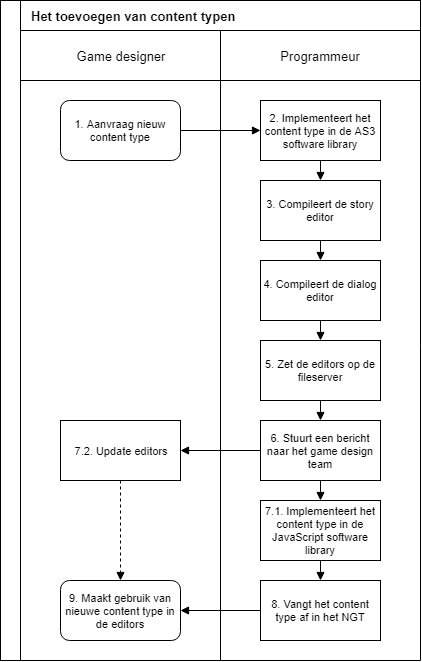
\includegraphics[width=0.38\textwidth]{Proces_ToevoegenContentTypeHuidig}
    \caption{Proces: het toevoegen van content types}
    \label{fig:procesaddcontenttypescurrent}
    \centering
\end{wrapfigure}
De editors maken gebruik van content types die gedefinieerd zijn in de \&ranj software library. In de software library bevinden zich klassen die ieder een content type vormen; content types hebben een statische definitie, ze zijn in de editor gebakken. Dit biedt wel meer controle over het content type, maar deze hoeveelheid controle is overtollig, content types blijven datastructuren. Hiernaast maakt dit het proces van het toevoegen en verwijderen van content types lastiger. Om dit te bereiken moet de broncode van de editor worden aangepast en vervolgens moet de editor opnieuw worden gecompileerd. Het huidige proces voor het toevoegen van een content type ziet eruit als in \autoref{fig:procesaddcontenttypescurrent}.

\begin{enumerate}
    \item De game designer wilt onderscheid maken tussen quiz tekst die gebonden staat aan een tijdslimiet en vragen die de hoofdpersoon zichzelf stelt, waarbij de speler geen tijdsdruk heeft. De game designer heeft aparte content typen nodig om onderscheid te maken tussen deze twee typen game content.
    \item De programmeur implementeert deze content typen in de \&ranj ActionScript3 (AS3) software library. Uit deze library halen de editors de content types. In de software library wordt aan gegeven welke editors gebruik mogen maken van het content type. Hieruit kan geconcludeerd worden dat er geen encapsulatie van content typen bestaat. De editors zouden zelf aan moeten geven van welke content typen ze gebruik maken.
    \item De programmeur haalt de nieuwe versie van de AS3 library binnen en past het versie nummer aan. Hierna compileert de programmeur handmatig de story editor.    \item Stap 3 wordt herhaald door de programmeur, maar dan voor de dialog editor.
    \item De installers van de vier editors worden op de file server van \&ranj gezet. Dit is een gedeelde folder waar medewerkers van het bedrijf toegang tot hebben.
    \item De programmeur stuurt een mail naar het game design team waarin staat dat er een nieuwe versie van de editors beschikbaar is. Hiernaast staan veranderingen en de locatie van de nieuwe editor in de mail.
    \item Terwijl de game designers de editors updaten (7.2), implementeert de programmeur het content type in de JavaScript software library, zodat deze gebruikt kan worden in het 'narrative game template' (NGT).
    \item De programmeur vangt het nieuwe content type af in het NGT en linkt deze aan de correcte actie.
    \item De game designer kan gebruik maken van het nieuwe content type. De game interpreteert het content type.
\end{enumerate}

\noindent De programmeur moet eerst de Apache Flex editor projecten opgezet hebben en daarnaast kennis hebben van deze projecten. Hiernaast moet de editor handmatig getest worden na het toevoegen van de nieuwe content typen om te kijken of deze nog werkt.
Een geautomatiseerde deployment pipeline zou kunnen helpen en veel werk uithanden nemen van de programmeur. Hiernaast moet het compilatie en deployment proces zoveel mogelijk vermeden worden, omdat dit tijd kost. Content typen blijven datastructuurtjes en het toevoegen of aanpassen van deze structuren zou geen compilatie van beide editors moeten vereisen.

\subsection{Misbruik van content typen}
Omdat het toevoegen of aanpassen van content typen een langdradig proces is wordt dit het liefst vermeden. Vaak worden er content typen uit oudere project misbruikt om onderscheid te kunnen maken tussen game content. Zo wordt ‘MinigameContent’ regelmatig gebruikt voor het tonen van hele andere dingen dan minigames.
Door content typen bij projecten op verschillende manieren te gebruiken kan er nooit op de eerste blik zeker gezegd worden wat voor doel het content type heeft.

\section{Flexibele selectie aan content typen}
Vanwege de diversiteit in game content verschillen de content typen sterk per project. De selectie aan content typen wordt geacht om dynamisch te zijn. Deze staan echter statisch gedefinieerd in de \&ranj AS3 software library. Er moet een manier komen om per project een selectie aan content typen te kunnen specificeren.
Een content type is een (kleine) datastructuur die bestaat uit een aantal velden. Zo bestaat ‘sms content’, een content type die een SMS vrij laat komen, uit een afzender, datum en inhoud. Door in ActionScript3 een type aan een veld toe te kennen kan er worden afgedwongen dat afzender en inhoud een tekst zijn en dat de datum een datum is. Vervolgens verbiedt de user interface foutief gebruik; de datum moet in een correct formaat staan. Restricties opleggen aan de user interface als validatie is gevaarlijk, want het is nog steeds niet zeker of de data valide is omdat deze mogelijk ook op andere manier kan ontstaan. Er wordt dus gezocht naar een oplossing waarmee velden in een content type gespecificeerd kunnen worden. Hiernaast moeten deze velden gevalideerd kunnen worden.

Om in het prototype een flexibele selectie aan content typen te kunnen specificeren wordt er gebruik gemaakt van een dataschema. Dit dataschema wordt uitgelezen wanneer het prototype opstart. Het schema kan aangepast worden om content typen te creëren, aan te passen of te verwijderen. Hiervoor hoeft het prototype niet opnieuw gebouwd te worden. Per project kan er gebruik gemaakt worden van een andere dataschema wat het inrichten van project specifieke content typen mogelijk maakt. De flexibiliteit van de nieuwe editor wordt sterk bevorderd door het niet continu te hoeven compileren van de editor om content typen de beheren. Daarnaast kunnen content typen per project gespecificeerd worden door voor ieder project een apart dataschema aan te maken en deze op te nemen in de overkoepelende projectstructuur (\autoref{ch:overkoepelendeprojectstructuur}). Dit gaat de vervuiling van de content typen scope tegen.

\begin{wrapfigure}{r}{0.5\textwidth}
    \fbox{
        \parbox{0.48\textwidth}{
            \textbf{SMSContent} bestaat uit\\
            een \textbf{afzender} weergeven in \textbf{tekst}\\
            een \textbf{ontvang datum} weergeven als \textbf{datum}\\
            een \textbf{inhoud} weergeven als \textbf{tekst}
        }
    }
    \caption{Pseudo dataschema voor 'sms content'}
    \label{fig:pseudosmscontent}
\end{wrapfigure}

\pagebreak
\noindent Om de velden van de content typen te specificeren zal er gebruik gemaakt worden van dataschema’s. Met dataschema’s kan er een set aan regels worden opgelegd aan de datastructuur. Hierbij is het belangrijk dat het zowel leesbaar is voor mens als machine. Een pseudo dataschema voor ‘sms content’ zou eruit kunnen zien als in \autoref{fig:pseudosmscontent}.
Dit pseudo dataschema is leesbaar voor mensen, maar niet voor computers. Computers hebben een gestandaardiseerd formaat nodig om data te kunnen interpreteren, zoals Extensible Markup Language (XML) of JavaScript Object Notation (JSON). In deze context is er gekozen voor JSON
Door gebruik te maken van een dataschema kan het proces voor het toevoegen van content typen sterk worden versimpeld. In het nieuwe proces, zoals weergeven in \autoref{fig:procesaddcontenttypesnew}, is het compileren en uitrollen van de editors niet meer nodig wanneer de selectie aan content typen aangepast moet worden.

\begin{figure}[htb]
    \centering
    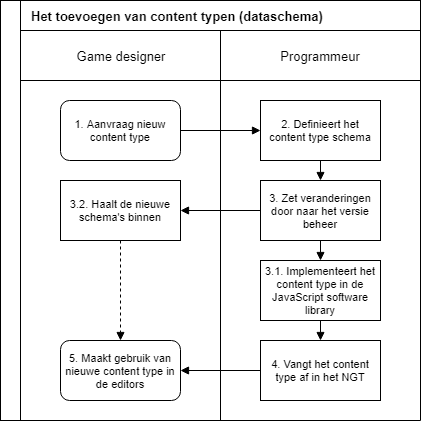
\includegraphics[width=0.52\textwidth]{Proces_ToevoegenContentTypeNieuw}
    \caption{Een versimpeld proces voor het toevoegen van content typen.}
    \label{fig:procesaddcontenttypesnew}
\end{figure}

\pagebreak
\subsection{JSON-dataschema}
JSON is een populaire keuze; het is klein en snel. Er kwam steeds meer vraag naar nieuwe functionaliteiten, zoals het kunnen specificeren van schema’s\cite{Severance2012}. 
Vanwege de vraag naar schema’s in JSON is het er een woordenboek opgezet waarmee JSON-schema’s opgezet kunnen worden\cite{JsonSchemaOrg}. In dit woordenboek staan afspraken over keywords en hun functionaliteit. Door gebruik te maken van deze keywords, met name type en properties, kan het schema voor ‘sms content’ wordt opgezet zoals in \autoref{lst:jsonschemasmscontent}. Het JSON-document in \autoref{lst:jsonsmscontent} is valide volgens het schema in \autoref{lst:jsonschemasmscontent}.

% \begin{figure}[htb]
    % \centering
    \lstset{language=JSON}
    \begin{lstlisting}[caption={JSON-schema voor 'sms content'.},captionpos=b,label={lst:jsonschemasmscontent}]
    {
        "type": "object",
        "properties": {
            "sender": {
                "type": "string"
            },
            "date": {
                "type": "string",
                "format": "date-time"
            },
            "content": {
                "type": "string"
            }
        }
    }             
    \end{lstlisting}    
    % \label{lst:jsonschemasmscontent}
% \end{figure}

% \begin{figure}[htb]
%     \centering
    \lstset{language=JSON}
    \begin{lstlisting}[label={lst:jsonsmscontent},caption={Valide JSON-document van 'sms content'.},captionpos=b]
    {
        "sender": "Harold",
        "date": "2018-04-21T11:00:00",
        "content": "Great moves, keep it up!"
    }                   
    \end{lstlisting}
% \end{figure}

\pagebreak
\section{Een schaalbaar dataschema voor content typen}
Hoewel XML beschikt over "out-of-the-box" dataschema functionaliteit is het gebruik van JSON preferabel. Niet alleen is het serialisatie proces van JSON sneller\cite{Nurseitov}, maar JavaScript biedt ook directe ondersteuning voor JSON. Hiernaast is het relatief makkelijk voor iemand die met JavaScript werkt om JSON te begrijpen. Een oorzaak hiervan kan zijn dat JSON JavaScript objecten representeerd. Tenslotte blijkt uit het naast elkaar leggen van de dataformaten (\autoref{app:contenttypeschemeinxml}) JSON veel kleiner te zijn dan XML.

\subsection{JSON-schema structuur}
Ieder JSON-schema beschikt over de volgende structuur:
\begin{itemize}
    \item \$schema; geeft aan dat een JSON-document een JSON-schema is. Hiernaast geeft de waarde aan welke schema versie dit schema voldoet\cite{Droettboom2016}. Dit kan ook een aangepast schema zijn dat afwijkt van het originele schema, om bijvoorbeeld, uitgebreide functionaliteit te ondersteunen.
    \item \$id; Definieert een Uniform Resource Identifier (URI) voor het schema. Deze URI kan gebruikt worden om te refereren naar het bijbehorende schema.
    \item title; Titel van het schema
    \item description; Omschrijving van het schema; waar het schema voor staat.
    \item definitions; Optionele sectie waarin schema definities geplaatst kunnen worden die in het daadwerkelijke schema hergebruikt kunnen worden\cite{FoundationsJSONSchema}.
    \item Het daadwerkelijk schema waartegen JSON-documenten gevalideerd worden. Een voorbeeld is terug te zien in \autoref{lst:jsonschemasmscontent}.
\end{itemize}

\subsection{Referenties}
Om het schema schaalbaar op te zetten zullen mogelijke properties van content typen gedefinieerd worden onder ‘definitions’. Een voorbeeld hiervan is terug te zien in \autoref{lst:contenttypejsonschemaexample}. Deze properties kunnen vervolgens worden (her)gebruikt in de daadwerkelijke content typen, door gebruik van het \$ref keyword\cite{Droettboom2016}. Dit keyword refereert naar een ander schema via het schema \$id.

% \begin{figure}[H]
%     \centering
    \lstset{language=JSON}
    \begin{lstlisting}[caption={Voorbeeld content type JSON-Schema.},captionpos=b,label={lst:contenttypejsonschemaexample}]
    {
        "$schema": "http://json-schema.org/draft-07/schema#",
        "$id": "http://www.ranjnet.nl/content#",
        "definitions": {
            "propertyTypes": {
                "stringProperty": {
                    "$id": "#/definitions/propertyTypes/stringProperty",
                    "type": "string",
                    "default": ""
                }
            }
        }
    }                            
    \end{lstlisting}
% \end{figure}

\noindent Met deze properties kan er een basis content schema worden opgezet. Deze bevat properties die in elk concrete content type terugkomen. In \autoref{lst:basecontentjsonschema} staat een voorbeeld van een simpel base content schema die gebruik maakt van de eerder gedefinieerde string property.

% \begin{figure}[htb]
%     \centering
    \lstset{language=JSON}
    \begin{lstlisting}[caption={JSON-schema van base content.},captionpos=b,label={lst:basecontentjsonschema}]
    {
        "baseContent": {
            "type": "object",
            "properties": {
                "type": {
                    "$ref": "#/definitions/propertyTypes/stringProperty"
                }
            }
        }
    }               
    \end{lstlisting}
% \end{figure}

\subsection{Combinaties}
Door een ‘base content’ schema te definiëren met properties die voorkomen in ieder content type schema wordt de grootte van het JSON-schema minimaal gehouden. Hergebruik van andere schema’s vergroot de schaalbaarheid van het schema.
Het ‘base content’ schema moet gecombineerd kunnen worden met de daadwerkelijke content types die gebruikt zullen worden in de editor en het NGT. Hiervoor maakt JSON-schema gebruik van het ‘allOf’ keyword. Een schema met het ‘allOf’ keyword is pas valide wanneer de onderliggende schema’s, gespecificeerd in ‘allOf’, valide zijn\cite{Droettboom2016}. Het schema in \autoref{lst:jsonschemaallofexample} definieert ‘text content’, welke valide is als de twee onderliggende schema’s valide zijn.
De ‘\$ref’ en ‘allOf’ keywords brengen complicaties met zich mee die in een later hoofdstuk besproken zullen worden.

% \begin{figure}[htb]
%     \centering
    \lstset{language=JSON}
    \begin{lstlisting}[caption={Een content schema die gebruik maakt van het 'allOf' keyword.},captionpos=b,label={lst:jsonschemaallofexample}]
    {
        "textContent": {
            "allOf": [
                {
                    "$ref": "#/definitions/baseContent"
                },
                {
                    "$id": "#/contentTypes/textContent",
                    "title": "Text content",
                    "description": "Textual content",
                    "properties": {
                        "text": {
                            "$ref": "#/definitions/propertyTypes/stringProperty"
                        }
                    }
                }
            ]
        }
    }
    \end{lstlisting}
    % \caption{Een content schema die gebruik maakt van het 'allOf' keyword.}
    % \label{fig:jsonschemaallofexample}
% \end{figure}

\section{JSON-schema integreren met de editor}
De properties van een content node kunnen worden aangepast door de gebruiker. Het selecteren van een content node resulteert in het tonen van de bijbehorende properties. De inspector (te zien in \autoref{fig:storyeditorinspector}) is verantwoordelijk voor het tonen van deze properties.

\begin{figure}[htb]
    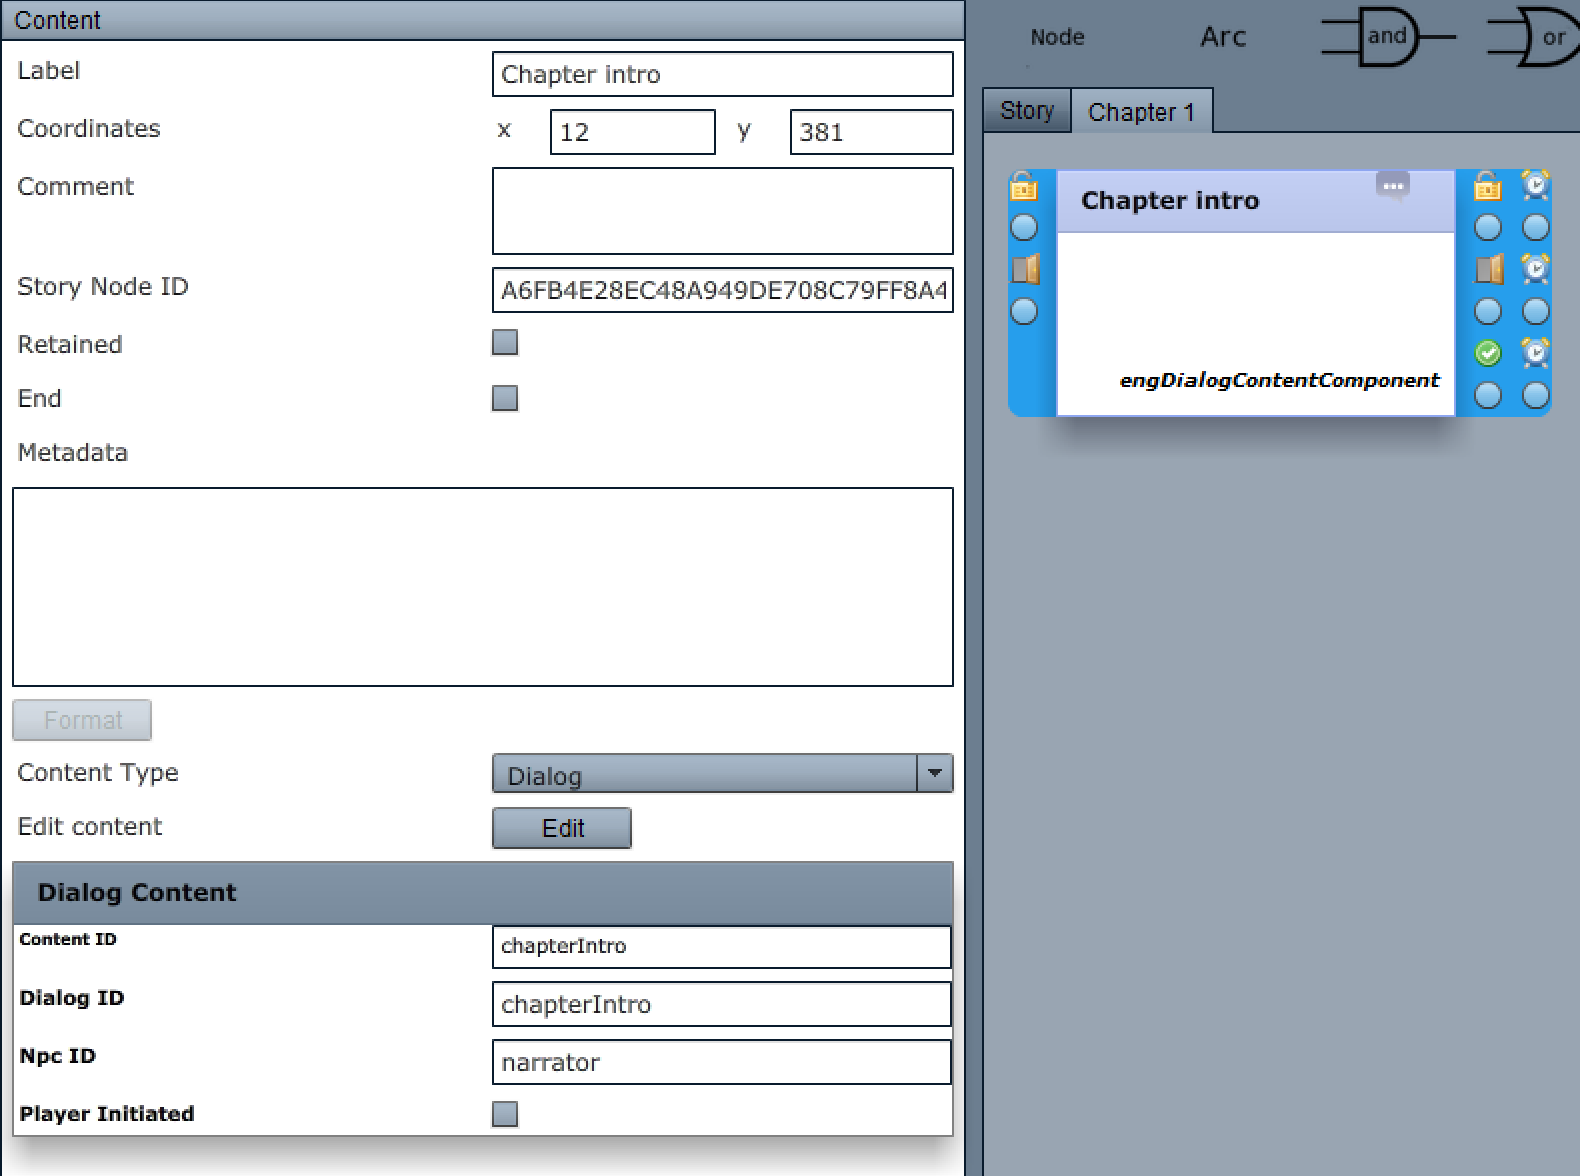
\includegraphics[width=\textwidth,height=\textheight,keepaspectratio]{StoryEditor_Inspector}
    \caption{De inspector die een geselecteerde dialog node toont.}
    \label{fig:storyeditorinspector}
    \centering
\end{figure}

In de nieuwe editor moet de inspector de properties tonen van het bijbehorende schema. Bij het opzetten van het content schema is er gebruik gemaakt van referenties om properties toe te kennen aan content typen. Dit resulteert in een schaalbaar JSON-schema, maar introduceert een probleem voor de inspector. Deze kan niet omgaan met referenties en combinaties van schema’s.

\subsection{Het content schema voorbereiden}
Om het content schema bruikbaar te maken voor de inspector moeten de volgende stappen worden ondernomen:

\begin{enumerate}
    \item Referenties resolven; ‘\$ref’ keywords vervangen door het daadwerkelijke gerefereerde object.
    \item Combinaties platslaan; ‘allOf’ keywords vervangen door een samenvoeging van onderliggende schema’s.
\end{enumerate}

Deze stappen moeten worden uitgevoerd wanneer de editor opstart, omdat het wenselijk is om deze functionaliteit te hebben bij het opzetten van het schema. De editor maakt dan een interne copy van het schema en zet deze om naar een schema zonder referenties en combinaties.

\subsubsection{Het oplossen van referenties}
Om referenties te resolven moet er eerst gekeken worden naar hoe het \$id keyword werkt. In de root, het hoogste niveau, van het JSON-schema wordt de locatie van het schema aangegeven. Het schema zelf dient toegankelijk te zijn op deze locatie om referenties vanuit andere schema’s toe te laten \cite{DraftJSONSchema07}. Binnen content type schema’s kan gebruik gemaakt worden van een hashtag (\#) om te refereren naar het root schema.

Als voorbeeld voor het resolven van referenties wordt er gekeken naar \autoref{lst:jsonschemrefexample}. Deze specificeert een schema voor ‘base content’ waarin gerefereerd wordt naar een ander schema, namelijk ‘string property’. Het pad van de referentie luidt: “\#/definitions/propertyTypes/stringProperty”. Hierin verwijst de hashtag naar de root van het schema: “http://www.ranjnet.nl/content”. Het bijbehorende object kan gevonden worden door vanaf de root te reduceren volgens het pad. Vervolgens wordt het \$ref keyword vervangen door het gevonden schema.
De community rondom JSON-schema leidt ook tot bestaande oplossingen zoals ‘json-schema-ref-parser’\footnote{https://github.com/BigstickCarpet/json-schema-ref-parser} en ‘json-schema-deref’\footnote{https://github.com/bojand/json-schema-deref }. Beide oplossingen zijn libraries die \$ref keywords resolven.


% \begin{figure}[htb]
%     \centering
    \lstset{language=JSON}
    \begin{lstlisting}[caption={Een JSON-Schema met referentie.},captionpos=b,label={lst:jsonschemrefexample}]
    {
        "$schema": "http://json-schema.org/draft-07/schema#",
        "$id": "http://www.ranjnet.nl/content#",
        "definitions": {
            "propertyTypes": {
                    "stringProperty": {
                    "$id": "#/definitions/propertyTypes/stringProperty",
                    "type": "string",
                    "default": ""
                }
            }
        },
        "baseContent": {
            "type": "object",
            "properties": {
                "type": {
                    "$ref": "#/definitions/propertyTypes/stringProperty"
                }
            }
        }
    }          
    \end{lstlisting}
    % \caption{Een JSON-Schema met referentie.}
    % \label{lst:jsonschemrefexample}
% \end{figure}


\subsubsection{Het platslaan van combinaties}
Combinaties gemaakt door het ‘allOf’ keyword kunnen worden platgeslagen door de onderliggende schema’s samen te voegen in één schema object. Er wordt een object gemaakt waarnaar de velden van de onderliggende schema’s gekopieerd worden. Dit proces begint bij het eerste onderliggende schema wat betekent latere schema’s eventuele al bestaande velden zullen overschrijven.
Hoewel deze stap nodig is om het schema bruikbaar te maken voor de inspector is het samenvoegen van onderliggende schema’s niet juist volgens de definitie van het ‘allOf’ keyword. Volgens JSON-schema is een schema met ‘allOf’ pas valide wanneer elk onderliggend schema valide is\cite{FoundationsJSONSchema}. Dit betekent dat onderliggende schema’s niks van elkaar af weten. Door onderliggende schema’s plat te slaan naar één schema wordt deze barrière gebroken wat leidt tot een overtreding van JSON-schema. Deze schending van JSON-schema regels kan leiden tot onverwacht gedrag in de inspector. Zo zou het JSON-schema in \autoref{lst:allofinvalidjsonschema} nooit valide kunnen zijn, omdat het 'allOf' kijkt naar zowel het 'person' als 'address' schema. Deze schema's bevatten allebei een 'identifier' property maar van een ander type. Hierdoor is ieder JSON-object dat gevalideerd wordt tegen dit schema invalide. Dit betekend dat de editor invalide JSON-schema's accepteert en kan tonen in de inspector. Daarom is het belangrijk om eerst het JSON-schema te valideren tijdens het opstarten van de editor.

% \begin{figure}[H]
%     \centering
    \lstset{language=JSON}
    \begin{lstlisting}[caption={Een invalide JSON-schema, door foutief gebruik van het 'allOf' keyword.},captionpos=b,label={lst:allofinvalidjsonschema}]
    {
        "$schema": "http://json-schema.org/draft-07/schema#",
        "definitions": {
            "person": {
                "$id": "#/definitions/person",
                "type": "object",
                "properties": {
                    "identifier": {
                        "type": "string"
                    }
                },
                "required": [
                    "identifier"
                ]
            },
            "address": {
                "$id": "#/definitions/address",
                "type": "object",
                "properties": {
                    "identifier": {
                        "type": "number"
                    },
                    "nr": {
                        "type": "number"
                    }
                },
                "required": [
                    "nr"
                ]
            }
        },
        "allOf": [
            {
                "$ref": "#/definitions/person"
            },
            {
                "$ref": "#/definitions/address"
            }
        ]
    }     
    \end{lstlisting}
% \end{figure}

\pagebreak
\subsection{Reflecteren van content types in de inspector}
De inspector moet het content type van een geselecteerde content node inzichtelijk en bewerkbaar maken. Bij ‘text content’ schema, die bestaat uit een string property, moet de inspector dan ook een tekstveld tonen waarmee de tekst in het content type kan worden aangepast.
\subsubsection{Primitieve types}
Omdat content types gedefinieerd zijn in JSON-schema’s, moet de inspector alle zes primitieve types\cite{Droettboom2016} ondersteunen om het schema te kunnen reflecteren. De selectie van primitieve types in JSON-schema bestaan uit:

\begin{enumerate}
    \item string
    \item boolean
    \item number
    \item object
    \item array
    \item null
\end{enumerate}

\noindent Ieder type heeft een eigen representatie. Met React kan de representatie van ieder type worden ingekapseld in componenten.

In \autoref{fig:representationschematypes} wordt een voorstel gedaan voor de representatie van de types\footnote{“null” heeft geen representatie}.

\subsubsection{Compositie}
Het voorstel in \autoref{fig:representationschematypes} maakt gebruik van een compositie structuur; types kunnen voorkomen in andere types. Zo komen de types ‘string’ en ‘number’ terug in het object type. Een compositie structuur bestaat uit een boom van ‘composites’ en ‘leaves’. Composite objecten bevatten andere composite- en leaf objecten (\autoref{fig:compositetree}), zo zijn de types ‘object’ en ‘array’ composities. Leaf objecten beheren geen onderliggende objecten. De boom is valide wanneer deze begint met een composite en eindigt met leaves.

\begin{figure}[H]
    \centering
    \begin{minipage}{.5\textwidth}
        \centering
        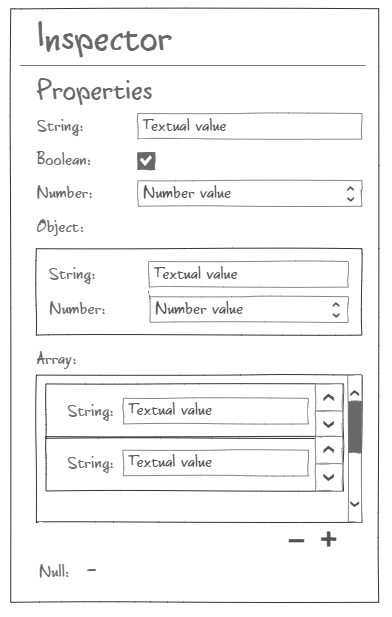
\includegraphics[width=.82\linewidth]{WireframeInspector}
        \caption{Representatie van primitieve JSON-schema types.}
        \label{fig:representationschematypes}    
    \end{minipage}%
    \begin{minipage}{.5\textwidth}
        \centering
        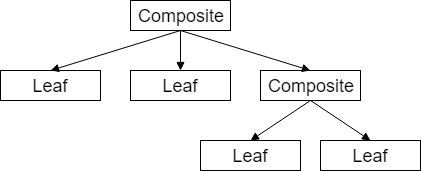
\includegraphics[width=.82\linewidth]{CompositeTree}
        \caption{Een valide compositie boom.}
        \label{fig:compositetree}
    \end{minipage}
\end{figure}

\subsubsection{Implementatie}
\begin{wrapfigure}{r}{0.42\textwidth}
    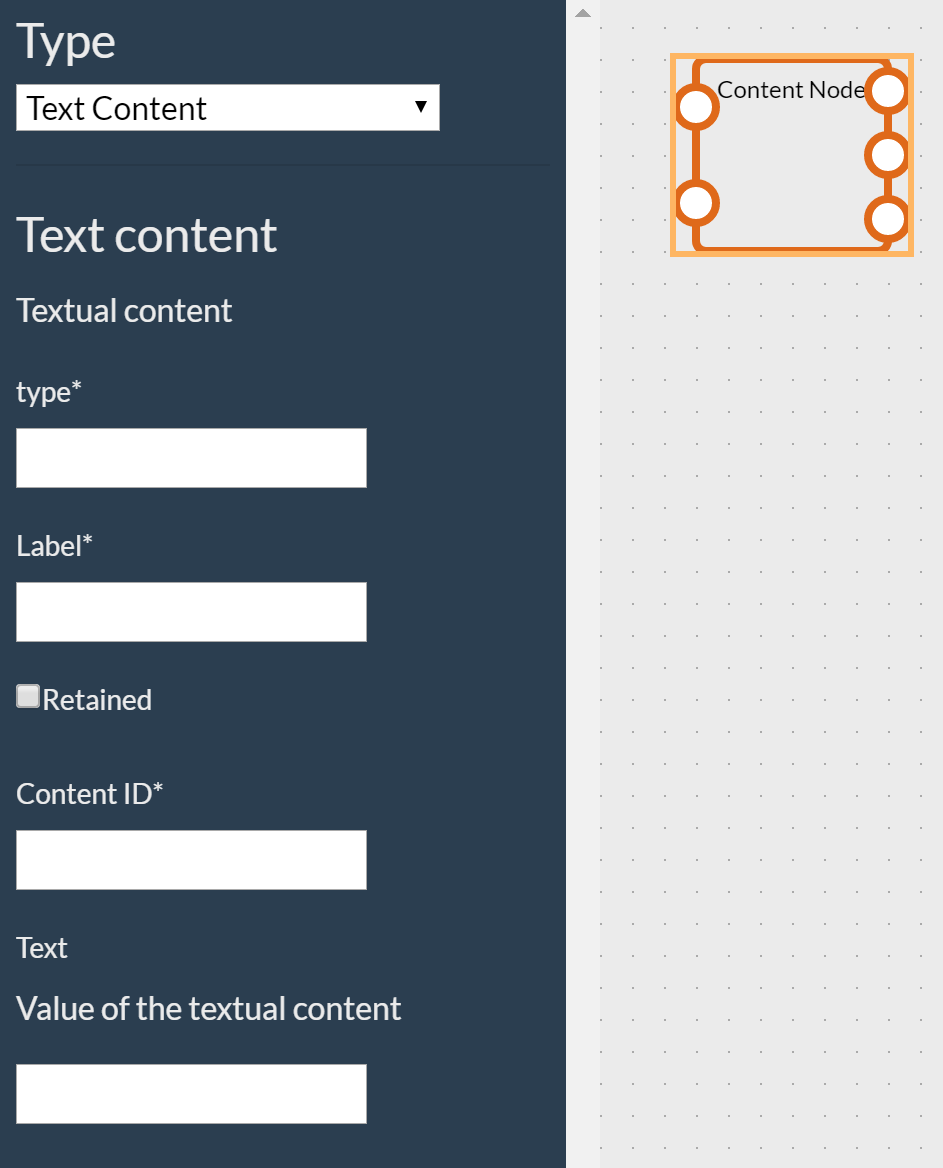
\includegraphics[width=0.41\textwidth]{PrototypeInspector}
    \caption{Het inspecteren van een content type in het prototype.}
    \label{fig:prototypeinspector}
    \centering
\end{wrapfigure}

In het prototype is er gebruik gemaakt van de ‘react-jsonschema-form’\footnote{https://github.com/mozilla-services/react-jsonschema-form/} library om JSON-schema om te zetten in HTML input elementen. Dit doet de library door een React component aan te bieden die een JSON-schema als parameter neemt. Bij iedere property wordt vervolgens een bijpassend HTML-element gezocht die getoond wordt in de inspector. In \autoref{fig:prototypeinspector} wordt het 'text content' schema van \autoref{lst:jsonschemaallofexample} getoond in de inspector van het prototype.

\pagebreak

\section{Conclusie}
Met deze conclusie wordt de deelvraag “Hoe kan diverse game content ondersteund worden?” beantwoord.

Diverse game content kan worden ondersteund door gebruik te maken van content typen. Het specificeren van content typen door middel van dataschema’s maakt het beheren van content typen mogelijk en draagt bij aan de flexibiliteit van de editors. JSON-schema is een licht en snel dataschema formaat geschreven in JSON. Door middel van referenties en combinaties kan er een schaalbaar dataschema worden opgezet. Omdat JavaScript JSON "out-of-the-box" ondersteunt is deze goed te integreren met de nieuwe technology stack die gebruik maakt van JavaScript. Hiernaast zijn er bestaande oplossingen in de vorm van libraries voor het valideren, manipuleren en reflecteren van JSON-schema’s.

\section{Vervolgonderzoek}
\paragraph{Vervuiling van de content typen selectie}
Om vervuiling van de content typen selectie te voorkomen zullen de JSON-schema’s deel uit gaan moeten maken van het project. Zo beschikt iedere game over een selectie aan content typen die voor haar relevant is. In de huidige situatie staan de editors los van de game engine. Om game content te kunnen bewerken die specifiek is voor een project zullen de editors opgenomen moeten worden in een overkoepelde projectstructuur. In \autoref{ch:overkoepelendeprojectstructuur} wordt een voorstel gedaan voor een overkoepelende projectstructuur.

\paragraph{JSON-schema combinatie keywords}
Met deze oplossing kan er geen gebruik gemaakt worden van andere combinatie keywords die JSON-schema biedt. Naast het ‘allOf’ keyword zijn er ook nog de combinatie keywords: ‘anyOf’, ‘oneOf’ en ‘not’.